\chapter{Shaping on HBT-EP}
\section{Hardware}
\subsection{The Coil}
\paragraph{} The shaping coil is a single continuous piece of 1/0 welding cable, run eight times toroidally between the inner ring of the toroidal field magnet cases and the vacuum vessel.  This ex-vessel coil is located slightly above the midplane, mainly due to space limitations.  Were there complete freedom of placement, the coil would likely be placed nearer the midplane, as we have active (pre-programmed) control of the plasma's radial location, but vertical location control is only passively provided by eddies in the conducting vessel walls and shells.  Further, placing the coil at the midplane would locate it closer the the plasma, increasing coupling and reducing the current requirements for any given shape
\subsubsection{Leads \& Bundle Connections} 
The construction of the coil out of a single conductor was accomplished through directing the conductor from one bundle to another once the number of required turns had been wound.  This necessitated a poloidal run of wire to connect the two.  At the end of the final bundle, the out-lead cable had to travel poloidally once again to meet the in-lead before becoming a twisted pair.  These non-toroidal runs of current were canceled to the best of our ability by running the return lead back at the same location as the poloidal leads connecting each bundle.  Though the thickness of the cable and the tight spaces involved precluded winding these contrary wires, they were connected with zip ties to ensure as good a canceling as possible.  See Figure 1 for a schematic of the windings and location of the leads.\\
\begin{figure}
\includegraphics[width = \textwidth]{./figures/Coil_winding_schematic.png}\begin{flushleft}
\caption{Schematic of the current direction, inter-bundle connections and coil leads, as seen by an observer between the vacuum vessel's inboard side and the coil.  The toroidal direction is left/right, poloidal is up/down.}
\end{flushleft}
\label{coil_winding}
\end{figure}
The twisted pair from the power supply rises from the laboratory basement, splits with one lead breaking into the lowest turn, and the other breaking out of the highest turn.  The top lead is therefore unshielded for roughly 8 inches.  There are two points at which the cable is bent back upon itself to begin a new bundle and reverse the direction of the current.  This occurs at the same toroidal location, which is itself the same location as the leads.  The current in the leads travels in the opposite direction from the current in the jumps between bundles.  The lead is thus lashed to the the interbundle connections to both reduce the error fields, and prevent the $\vec{j} X \vec{B}$ forces on the cables from causing damage to the coil insulation.
\subsubsection{The Power Supply}
\paragraph{}The shaping coil is energized by a pre-programmed two-stage passive capacitive supply.  A 7.5mF, 900V (max) bank provides the startup current, with a time to peak current of $800\mu s$.  As this bank discharges, a high current diode passively switches a second 'crowbar' bank into the circuit.  This bank has a capacitance of 0.6F, and a maximum voltage of 250V.  This much larger bank is capable of providing current enough to sustain a 'flat top' current pulse of $\sim$8kA for $\sim$5ms.  By selecting different voltages on each bank pre-discharge, a variety of different current profiles can be developed.  The 'soft start' of the crowbar bank due to the used of a diode allows for a very smooth transition between the two power banks.  This is compared to the current trace of the vertical field coil in Figure .  The power supplies for all other equilibrium field coils are capacitive in nature, but are switched in by ignitrons, which require a voltage drop between the bank and the line into which they switch the bank.  The rapid inrush current as a capacitor is switched into a line of a different voltage leads to a sharp change in the current, leading to strong eddies induced in the surrounding conducting structures.  The banks are easily charged to their full voltage in less than one minute, much less time than the other equilibirum field coil banks.  There are a variety of safety measures used in the bank's construction.  A discussion, full partslist and circuit schematic can be found in Appendix BLANK
\subsubsection{The Coil Holders}
The coil is supported against gravity and Lorentz forces by a set of ten  G-10 fiberglass/epoxy composite supports, which are themselves bolted to the TF cases.  The bolts are structural bolts, that had been used to clamp the TF cases shut.  Nuts located at the point of attachment have been removed, and the bolts instead thread into tapped holes in the supports.  The previous torque of 40 ft-lbs is applied, with no ill effects on the G-10 holder mounts, thus providing the same clamping force and avoiding any leaks of insulating oil.
These holders consist of two parts epoxied together, and thus do not disassemble.  The holders were attached to the Tokamak, and the coil was threaded sequentially through each hole in each conductor.  As such, any modifications or repairs to the coil or any locations on the tokamak obstructed by the coil will require the coil to be cut, or completely unwound.  Unwinding represents 2-3 business days of work, but cutting may make it difficult to splice and insulate the coil given the tight confines of its run.
The coil holders are further supplemented by a set of ten clamps, which hang from the coil itself.  Though they provide no resistance to gravity or external magnetic forces, they do prevent the coil's bundles from jumping apart due to the magnetic repulsion between the oppositely-directed bundles.
\subsubsection{Rip-testing of Coil Jump-out}
 
\subsubsection{The Material Limiter}
\paragraph{}The poloidal array sensors are protected by $\frac{1}{16}$'' stainless steel shimstock to protect against damage to the wires or ablation of the plastic forms by plasma impinging.  Under normal operating conditions the last closed flux surface of the plasma is 5mm radially inward from the surface of the sensors' shielding.  The plasma is in general vertically centered on the midplane, moves mostly radially, and disrupts inward, so sensors at the midplane are further protected by the inboard limiter, which establish a 5mm separation between plasma and sensors, and have much larger thermal mass than the shims that cover the sensors.
\paragraph{}However, this is not the case for sensors higher up that are near the location of the X-point.  These sensors which lack the extra protection of a limiter will see the steady state power flux increase as plasma will be preferentially exhausted along a cone expanding radially outward from the X-point.  Additionally, during disruptions, there will be an upward component to the forces on the plasma.  To ensure that this additional heat load does not cause harm to the sensors, a new set of 1/4" 316 stainless steel limiters was machined and installed.  These 'blade' limiters are attached by hex nuts to threaded rods spot welded to the flanges of the chamber pieces.  These limiters trace an arc concentric with the poloidal array sensors, and extend radially inward 5mm from the inner edge of the sensors.  Protection from plasma impingement is provided from $180^{\circ} \leq \Theta \geq 120^{\circ}$.

\begin{figure}
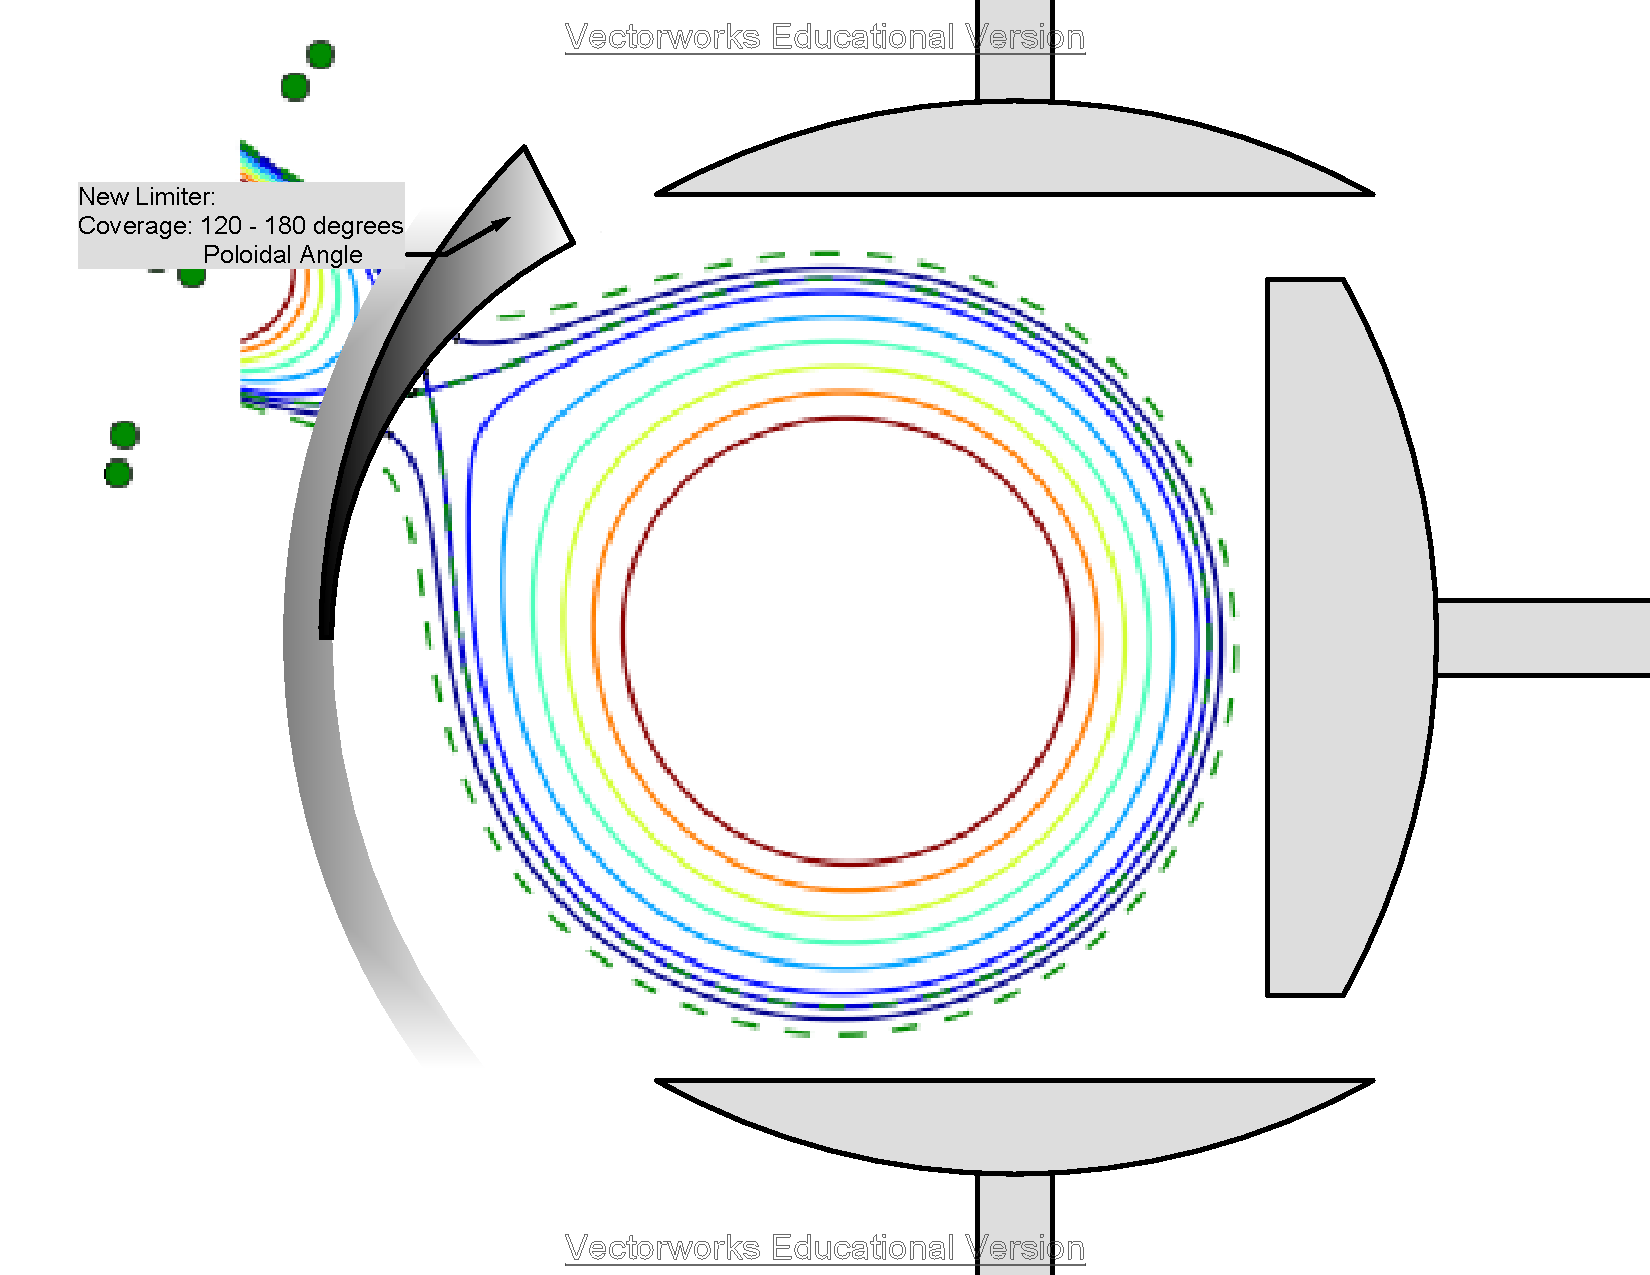
\includegraphics[width = \textwidth]{./figures/Poloidal_Cross_Section_shaping_plus_new_limter_v2013.pdf}\begin{flushleft}
\caption{Poloidal cross section of shaped plasma in chamber and limiting surfaces, with new limiter included.  Limiter is designed to to be conformal to a 15cm minor radius, inboard limited plasma.}
\end{flushleft}
\label{new_limiters}
\end{figure}

\subsection{Defining the Plasma Shape}
The definitions set out in \cite{Luce} will be used for discussion of the plasma shape in this research.  These definitions are more suited to the HBT-EP plasma, since the shaped equilibrium has no symmetry in the R-Z plane.  Common figures of merit, such as elongation and triangularity, can be defined for arbitrary geometries, and an analytic form for the LCFS can be derived.

The plot below shows a circular HBT-EP plasma, and a diverted plasma, with other equilibrium parameters (MR, I$_p$ being held constant) 